\documentclass{standalone}

\usepackage{tikz}
\usepackage{pgfplots}
\usepgfplotslibrary{statistics}
\usetikzlibrary{pgfplots.statistics}
\usepackage{etoolbox}

\newtoggle{label}
\togglefalse{label}

\pgfplotsset{compat=1.12}

\begin{document}
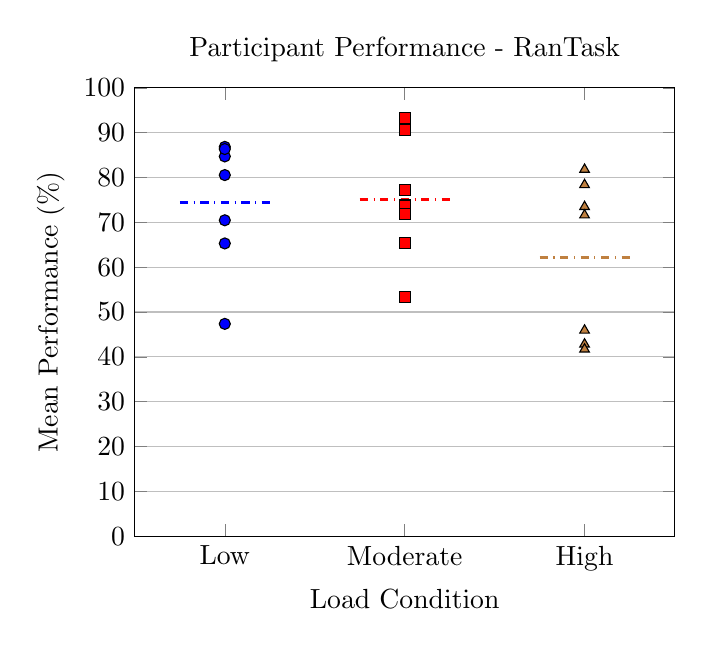
\begin{tikzpicture}
\begin{axis}[
	ymajorgrids,
	scatter/classes= {
		a={mark=*, fill=blue, draw=black},
		b={mark=square*, fill=red, draw=black},
		c={mark=triangle*, fill=brown, draw=black},
		d={mark=diamond*, fill=gray, draw=black}
	},
	ymin=0,
	ymax=100,
	xmin=.5,
	xmax=3.5,
	ytick={0,10,...,100},
	xtick={1,2,3},
	xticklabel style={align=center},
	xticklabels={Low, Moderate, High},
	title=Participant Performance - RanTask, 
	ylabel=Mean Performance (\%),
	xlabel=Load Condition]
	
	
	% Low
	\addplot+[ scatter,
			only marks,
			scatter src=explicit symbolic]
	coordinates {
			(1, 84.71)	[a]
			(1, 65.30)	[a]
			(1, 86.84)	[a]
			(1, 70.47)	[a]
			(1, 47.36)	[a]
			(1, 86.36)	[a]
			(1, 80.55)	[a]
};
\addplot+[ mark=None, dashdotted, blue, line width = 1pt ] 
	coordinates {
		(0.75, 74.51)
		(1.25, 74.51)
};

	% Moderate
	\addplot+[ scatter,
			only marks,
			scatter src=explicit symbolic]
	coordinates {
			(2, 73.75)	[b]
			(2, 77.30)	[b]
			(2, 90.70)	[b]
			(2, 65.48)	[b]
			(2, 53.43)	[b]
			(2, 93.31)	[b]
			(2, 71.79)	[b]
};
\addplot+[ mark=None, dashdotted, red, line width = 1pt ] 
	coordinates {
		(1.75, 75.11)
		(2.25, 75.11)
};

	% High
	\addplot+[ scatter,
			only marks,
			scatter src=explicit symbolic]
	coordinates {
			(3, 42.82)	[c]
			(3, 45.92)	[c]
			(3, 41.70)	[c]
			(3, 73.48)	[c]
			(3, 78.38)	[c]
			(3, 81.79)	[c]
			(3, 71.62)	[c]
};
\addplot+[ mark=None, dashdotted, brown, line width = 1pt ] 
	coordinates {
		(2.75, 62.24)
		(3.25, 62.24)
};


\end{axis}
\end{tikzpicture}

\end{document}
















